\documentclass[10pt,conference,compsocconf]{IEEEtran}

\usepackage{hyperref}
\usepackage{graphicx}
\usepackage[]{algorithm2e}
\usepackage{placeins}

\begin{document}
\title{Machine Learning - Project 1}
\author{
  Arnaud Pannatier - 
  Bastian Nanchen - 
  Matteo Giorla\\
  \textit{Group : }Max and Lily learn ML \\
  \textit{EPFL 2017}
}
\maketitle

\begin{abstract}
The goal of this project is to characterize events measured by CERN colliders to detect Higgs bosons which play a fundamental role in particles physics. Using machine learning methods we achieved to classify the CERN measures with an 83\% accuracy.

\end{abstract}

\section{Introduction}

All the data measured at the CERN the last three years takes about 100 petabytes \cite{CERN}. To treat this huge amount of data, state of the art algorithms are required. Machine Learning methods are particularly well suited for this kind of problems.

\section{The Structure of a Paper}

\begin{description}
\item[ML Methods] \ \\
  The 6 traditional machine learning methods.
\item[Our approach] \ \\
  An explanation of the preprocessing we did and details on some techniques we used in our code.
\item[Procedure] \ \\
  A summary of the steps from raw data to the results.
\item[Results] \ \\
  A comment on the results and possible improvement.
\end{description}


\section{ML Methods seen in Class}

\subsection{Linear regression using gradient descent}
To achieve good linear regression, the loss function must be minimized. In this case the considered loss function is the mean square error (MSE). To minimize it we apply the gradient descent process which is an iterative process that improves the weight vector at each step by moving in the opposite direction of the computed gradient. 

\subsection{Linear regression using stochastic gradient descent}
The same principle as in the first method is used, but instead of computing the gradient at each step, which is very expensive, we move forward multiple steps by selecting an approximation of the gradient. This approximation is computed using a random batch of indices.

\subsection{Least squares regression using normal equations}
Another way of computing the optimum of the loss function is to solve it analytically. It is not always possible but it works well with linear regression using mean square error : the process of optimization becomes in this case equivalent to solving a linear system of equations called \textit{normal equations}. In some cases, the implementation of these methods causes some trouble : if some of the columns are nearly collinear, the matrix of this system is ill-conditioned and leads to big numerical errors. To take this phenomenon into account some preprocessing of the data is applied and singular matrix errors are treated differently.

\subsection{Ridge regression using normal equations}
In order to have a simpler and more meaningful model, it is convenient to penalize the complicated models directly in the cost function. This is done by adding a \textit{regularization} term $\lambda \vert\vert w \vert\vert ^2$. Fortunately \textit{normal equations} of this particular problem can be computed as well. Solving it is called \textit{ridge regression}.

\subsection{Logistic regression using gradient descent}
The \textit{MSE loss function} is in theory not very well suited for binary classification. To recall the process, in binary classification the model gives predictions that are quantified by two values using a threshold process. As the predicted value can become very large before the quantization, they contribute a lot more to the \textit{square loss error} than their final value. To take these considerations into account, the \textit{logistic function} is used to transform the prediction into a value between 0 and 1. Naturally this transformation will induce an other loss function and therefore a new gradient function. The gradient descent process is then used to find the optimal weights. In some cases, the value of the weights can be large, so computing the exponential leads to overflow errors in the \textit{logistic function}. In order to solve this problem, the following equivalent function is used : 
\begin{equation}
f(x) = \frac{1}{2}+\frac{1}{2}\tanh \left(\frac{x}{2}\right)
\end{equation} 

\subsection{Regularized logistic regression using gradient descent}

As in the case of \textit{ridge regression}, it's often more meaningful to have smaller values for the weights. To take this into account, a \textit{regularization parameter} $\lambda \vert\vert w \vert\vert ^2$ is added to the loss function. Its gradient is then computed and the gradient descent process is used for the optimization.

\section{Our Approach}

\subsection{Preprocessing and data cleaning}
We tried to clean up the data by removing the meaningless variables (whose value is -999). To do so we first noticed that the data could be clustered into 4 groups defined by their \texttt{PRI\_jet\_num} value (which can be 0, 1, 2 or 3). This attribute defines how many "jet of particles" were detected by the collider. For each of the groups the same attributes are set to -999, since for example, if only one jet was detected the data of the second jet would logically be meaningless. After grouping the data into these 4 clusters we removed collinear columns since they would not have any incidence on the regression and would even get in our way when trying to compute the least squares and ridge regressions.

We tried using standardization of the columns but it appeared that it gave us slightly worse results.

\subsection{Cross-validation and better evaluation function}
In order to see the improvement, the cross-validation process was employed. In this way, we could see if at some point the data was overfitted by the model. To get a more meaningful evaluation function of the model, we created a function that return the percentage of good predicted entries. Combine with cross-validation, this tools really helped finding what was our best model.

\subsection{Feature engineering}
To get better results, we had the idea to fit the features not just linearly but with higher degree polynomials. To achieve this purpose, we extend the data by adding multiple times the data matrix at increasing powers, we also added the product between columns. The risk was at certain point to overfit the data, but we could see this limit by using the cross validation. 

\subsection{Model comparison}
The different methods were used to get prediction from the data. Their efficiency were evaluate using the evaluation function. Only two given adequate results : \textit{least square} and \textit{ridge regression}. Sadly the four other needed fine tuning in order to work well and even with that they did not improve the results. 

\section{Procedure}

\begin{algorithm}[h]
\DontPrintSemicolon
\KwData{The CSV file containing the data to classify}
 \KwResult{Predictions}
 Data is clustered into 4 groups as explained in the \textit{Preprocessing and data cleaning} subsection\;
\For{Degrees up to 13}{
Feature engineering (extending the matrix with additional degrees) \;
\For{Each of the 4 groups} {
\For{Subgroup in cross validation} {
Select best lambda and apply ridge regression\;
}
Remember the best prediction\;
}
}
Recombine the data of all groups\;
Return the prediction\;
\end{algorithm}

\section{Results}
As mentionned in the \textit{Preprocessing and data cleaning} subsection standardization didn't give good result and lead to the 2 score falls in submissions 3 and 6.

The table below explains the different steps we took to improve the predictions accuracy and the corresponding score.

\begin{figure}[h]
  \centering
  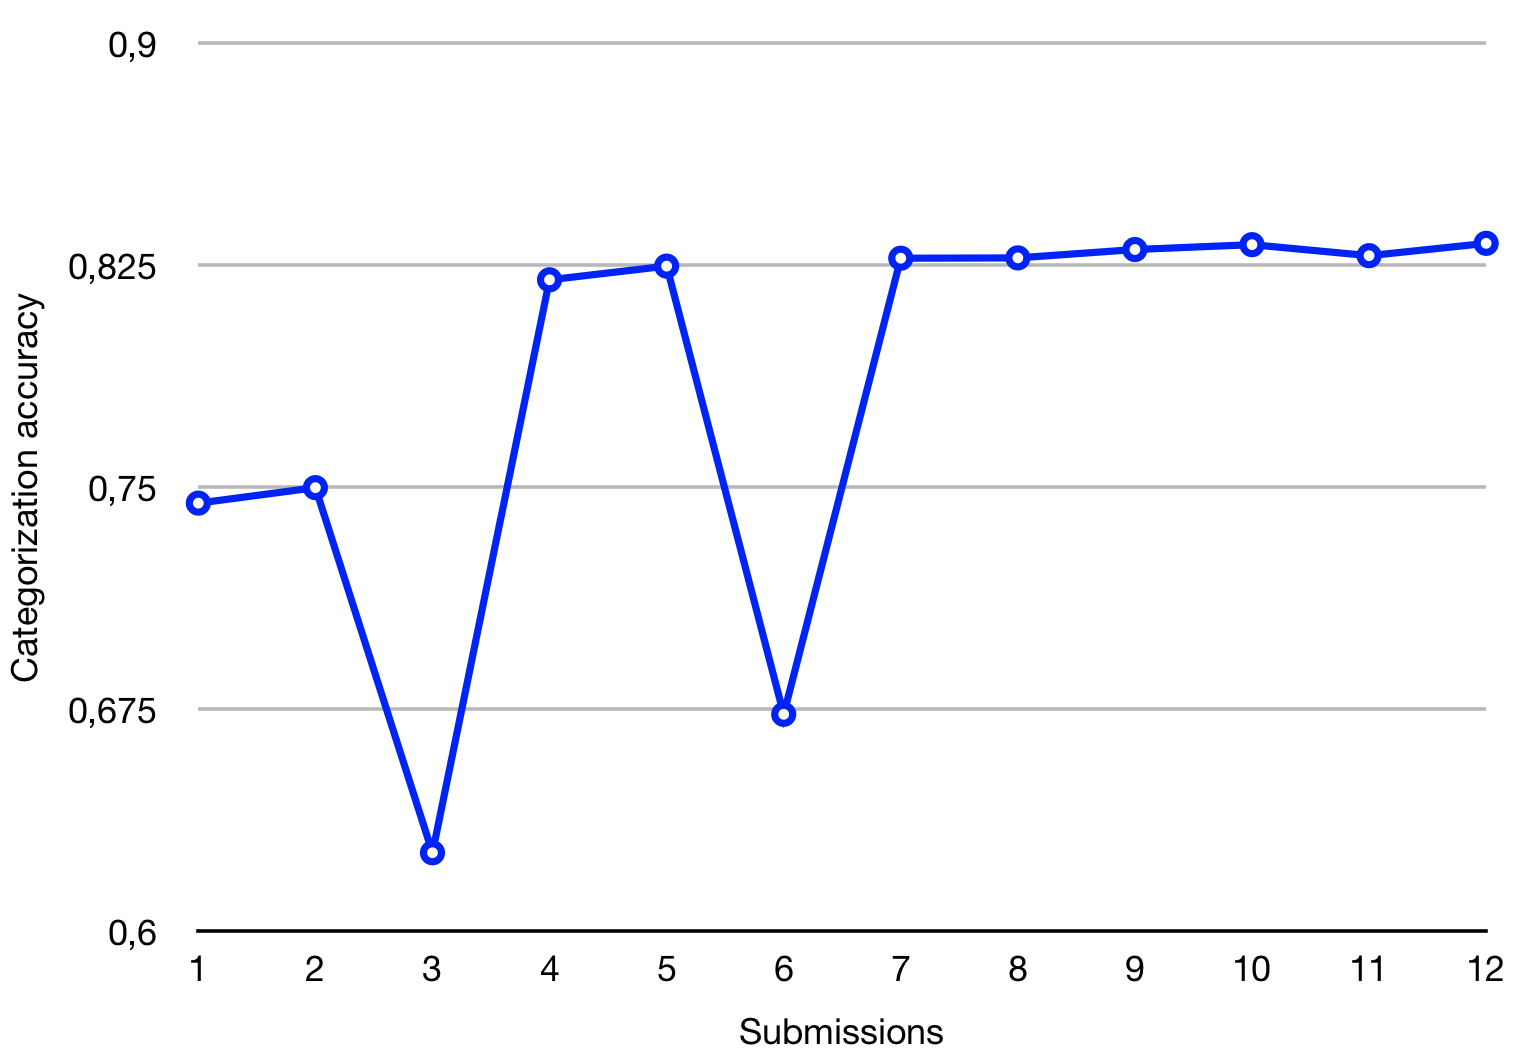
\includegraphics[width=\columnwidth]{graph}
  \caption{Progression of score.}
\end{figure}
\FloatBarrier

\begin{figure}[h]
  \centering
  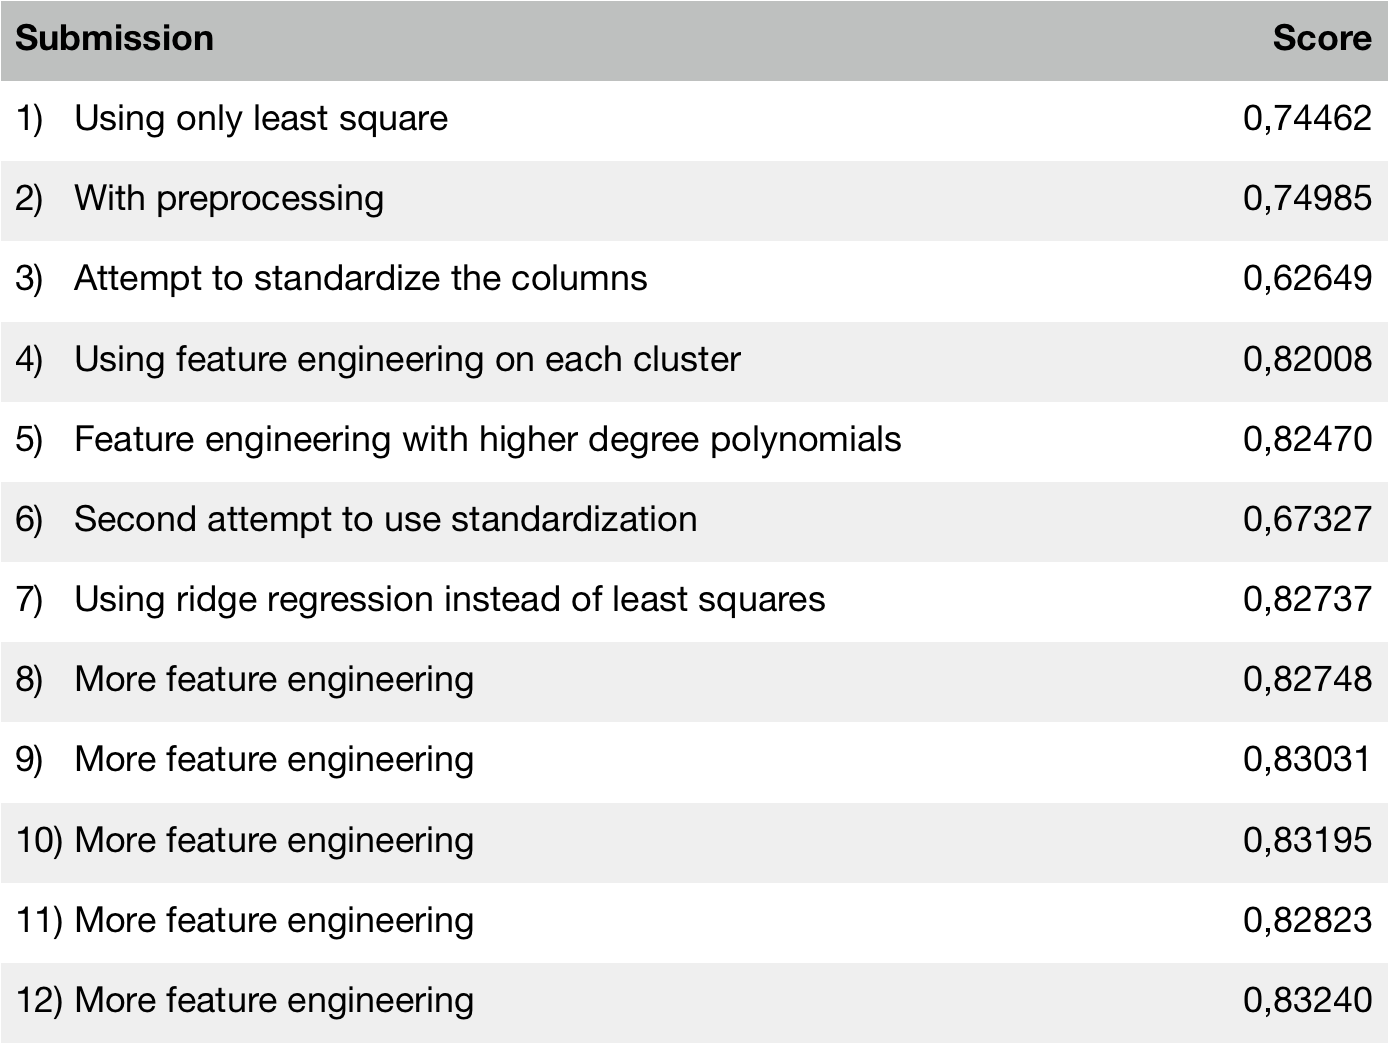
\includegraphics[width=\columnwidth]{table}
  \caption{Description of the progression of score.}
\end{figure}
\FloatBarrier


\section{Conclusion}
Machine Learning methods coupled with feature engineering have given great results as more of 83\% of the entries have been well categorized. In particular \textit{ridge regression} was well suited for this data set, and the best improvement in the categorization process was observed when the data was fitted with polynomials.

A lead to investigate to improve the results would be to find a specific way to increase the prediction quality for the group with \texttt{PRI\_jet\_num = 1} since this cluster currently has an accuracy rate of ~80\% in comparison to the overall result of more than 83\%.


\begin{thebibliography}{9}
\bibitem{CERN}
Cian O'Luanaigh, \textit{Le centre de donn�es du CERN franchit les 100 p�taoctets} \\
consulted the 28.10.17 at \url{https://home.cern/fr/about/updates/2013/02/cern-data-centre-passes-100-petabytes}
\end{thebibliography}


\end{document}


